% !TEX root = ../latex-faq-cn.tex

\let\fancybreak\relax

\section{数学公式(一)}
\label{sec:math-i}

%TODO: General

\faq{不带编号的行间公式为什么推荐使用 \cs{[}\ldots\cs{]} 而不是
  \texttt{\$\$}\ldots\texttt{\$\$}?}{display-math-env}

|$$|\ldots|$$| 是 \TeX{} 的用法,不适合在 \LaTeX{} 中使用。在 \LaTeX{} 中,\cs{[}\ldots\cs{]} 虽然
底层仍然依靠 |$$|\ldots|$$| 实现,但显然更加容易控制,也更容易实现特殊效果(例如靠左对齐)。

在 \pkg{amsmath} 宏包中,\cs{[}\ldots\cs{]} 被重定义为 \env{equation*} 环境的简写,它的实现比
\LaTeX{} 本身更好。所以我们建议,排版数学公式时始终调用 \pkg{amsmath} 宏包。

\begin{reference}
  \item 李清.\LaTeX{} 中不带编号的行间公式为什么推荐用 \cs{[}\ldots\cs{]} 而不是 |$$|\ldots|$$|?.
    \url{https://www.zhihu.com/question/27589739/answer/37255728}
  \item \url{https://tex.stackexchange.com/q/503}
  \item \url{https://tex.stackexchange.com/q/40492}
\end{reference}


\faq{如何让长公式自动断行?}{break-long-equation}

对于行内公式,一般来说 \LaTeX{} 会倾向于在二元运算符($+$、$-$ 等)和二元关系符($=$、$>$ 等)之后
断行,因此可以用 $F(x) \cdot G(x) \cdot H(x)$ 来代替 $F(x)G(x)H(x)$ 以允许换行。另外,我们建议把
列表项写成如 |$a$, $b$, $c$| 的形式而非 |$a, b, c$|,这样也可以避免出现糟糕的效果。

对于行间公式,可以使用 \pkg{amsmath} 宏包提供的一系列环境来手动断行:
\begin{itemize}
  \item \env{gather} 和 \env{gather*}:居中对齐
  \item \env{align} 和 \env{align*}:在 |&| 指定的位置对齐
  \item \env{multiline} 和 \env{multiline*}:首行左对齐,末行右对齐,中间居中
  \item \env{split}:类似 \env{align},在 |&| 指定的位置对齐,但需放在其他数学环境中使用
\end{itemize}
这里带 |*| 的版本表示不加编号。以上这些环境用法都是类似的,即在断行处加 |\\|。

公式的断行往往需要考虑语义因素,需要正确处理间距、对齐等,因此自动断行比较困难。\pkg{breqn} 宏包
提供了自动断行的可能,但有时候会出现兼容性问题,需要小心使用。

\begin{reference}
  \item 刘海洋.《\LaTeX{} 入门》 4.4~节、4.5.3~小节
\end{reference}


\faq{公式如何靠左(靠右)对齐?}{equation-left-right-align}

公式靠左对齐在基础文档类中由 |fleqn| 选项控制。选择该选项后,正文公式均靠左对齐,并且具有固定缩进
(由 \cs{mathindent} 控制)。至于(全局)靠右对齐,并没有直接的解决方案。

如果只需要部分公式靠左或靠右对齐,可以用 \env{flalign} 或者 \env{flalign*} 环境:

\begin{texlist}
  \begin{flalign}
    \int \sin x \, \mathrm{d} x = -\cos x + C & &
  \end{flalign}
  \begin{flalign}
    \int \cos x \, \mathrm{d} x = \sin x + C & &
  \end{flalign}
  \begin{flalign}
    & & \int \tan x \, \mathrm{d} x =  \ln |\sec x| + C
  \end{flalign}
\end{texlist}

\env{flalign} 环境本身用来实现分散对齐。因此用 |&&| 构成空列,就可以实现靠左或靠右对齐的效果:
\begin{flalign}
  \int \sin x \, \mathrm{d} x = -\cos x + C & &
\end{flalign}
\begin{flalign}
  \int \cos x \, \mathrm{d} x = \sin x + C & &
\end{flalign}
\begin{flalign}
  & & \int \tan x \, \mathrm{d} x =  \ln \vl\sec x\vl + C
\end{flalign}

\begin{reference}
  \item \url{https://tex.stackexchange.com/q/16840}
\end{reference}

\faq{怎样在大括号后给每个公式编号?}{}

可以借助 \cs{cases} 包的 \env{numcases} 环境,下面给出一个例子:

\begin{texlist}
  \documentclass{article}
  \usepackage{cases}
  \begin{document}
  \begin{numcases}{|x|=}
    x, & for $x \geq 0$\\
    -x, & for $x < 0$
  \end{numcases}
  \end{document}
\end{texlist}

\faq{公式希腊字符如何加粗?}{}

希腊字母没有原生粗体,可以使用 \pkg{bm}宏包中的 |\bm| 命令,
或者\pkg{unicode-math}宏包\footnote{需指定OpenType Math font,源代码文字为UTF8编
  码,直接输入希腊文。此包不能与其他一些math包共存。}中的|\symbf|或者其他伪粗命令。
\begin{reference}
  \item stackexchange. How can I get bold math symbols?. \url{https://tex.stackexchange.com/questions/595/how-can-i-get-bold-math-symbols}
\end{reference}

\faq{极限符号下面有两个趋近该怎么写}{}

可以使用\cs{atop},如:

\begin{texlist}
  \documentclass{article}
  \usepackage{mathtools}
  \begin{document}
  \begin{equation*}
       \lim_{n\to\infty\atop m\to\infty}
  \end{equation*}
  \end{document}
\end{texlist}

或者使用 \cs{substack},代码如下:

\begin{texlist}
  \documentclass{article}
  \usepackage{mathtools}
  \begin{document}
  \begin{equation*}
       \lim_{\substack{n\to\infty\\ m\to\infty}}
  \end{equation*}
  \end{document}
\end{texlist}
 
\faq{怎样在 LaTeX 中输入引号}{}

左引号用 |`|(键盘1旁边那个键),右引号用 |'|(正常输入单引号)。
西文双引号分别使用两次|`|和|'|。
中文条件下应直接使用中文双引号。
\begin{reference}
  \item 中华人民共和国教育部. 夹用英文的中文文本的标点符号用法(草案).\url{http://www.moe.gov.cn/s78/A19/yxs_left/moe_810/s230/201001/t20100115_75604.html}
\end{reference}

\faq{align 环境默认是居中对齐吗?我在使用时,发现公式开始是居中的,后来却一直靠右断对齐,这是什么原因?}{}

align环境采用的是奇偶对齐的方式,第一列右对齐,第二列左对齐,就这样右左右左依此类推,
两列之间用\&分隔。
给出一个使用它的例子:

\begin{texlist}
  \documentclass{article}
  \usepackage{amsmath}
  \begin{document}
  \begin{align}
    a_{11}& =b_{11}&
    a_{12}& =b_{12}\\
    a_{21}& =b_{21}&
    a_{22}& =b_{22}+c_{22}
  \end{align}
  \end{document}
\end{texlist}

\faq{公式已经有一个大括号了,还想在其中再加大括号,并且每个大括号有一个编号和内部公式尽量对其,该怎么实现?}{}

可以考虑使用 numcases 环境、aligned 环境、\textbackslash left\textbackslash \{、\textbackslash right. 和 \textbackslash hphantom 的组合。直接给出例子:

\begin{texlist}
  \documentclass{article}
  \usepackage[a4paper,margin=1in]{geometry}
  \usepackage{amsmath,cases}
  \begin{document}
  \begin{numcases}{}
    \left\{
    \begin{aligned}
      i = 1, 2, \dotsc, n, & \ j=1, \ a_{ij}=1\\
      & \ j = 2, \ a_{ij} = ( x_{T_i} - x_T )\\
      & \ j = 3, \ a_{ij} = ( t_{T_i} - t_T )\\
      & \ j = 4, \ a_{ij} = ( x_{T_i} - x_T )^2\\
      & \ j = 5, \ a_{ij} = ( x_{T_i} - x_T ) ( t_{T_i} - t_T )\\
      & \ j = 3, \ a_{ij} = ( t_{T_i} - t_T )^2\\
    \end{aligned}
    \right.\\
    \left\{
    \begin{aligned}
      i = n+1, n+2, \dotsc, 2n, \dotsc, n(n-1), & \ j = 1, 2, 3, 5, \ d_{ij}=0\\
      & \ j = 4, 6, \ \hphantom{3,5} \ d_{i,j}=1\\
    \end{aligned}
    \right.\\
    \left\{
    \begin{aligned}
      i = n(n-1) + 1, n(n-2) + 2, \dotsc, n^2,& \ j = 1, 2, 4, \ g_{ij} = 0\\
      & \ j = 3, \hphantom{,2,4} \ g_{ij} = 1\\
      & \ j = 5, \hphantom{,2,4} \ g_{ij} = (x_{T_k} - x_T) \ k=1,2,\dotsc,n\\
      & \ j = 6, \hphantom{,2,4} \ g_{ij} = 2 ( x_{T_k} - x_T ) \ k=1,2,\dotsc,n\\
    \end{aligned}
    \right.
  \end{numcases}
  \end{document}
\end{texlist}

\faq{如何产生不带编号的定理环境}{}

使用 amsthm 的 \cs{newtheorem*} 命令即可。下面给出 MWE
\begin{texlist}
  \documentclass{article}
  \usepackage{amsthm}
  \newtheorem*{thm*}{Theorem}
  \begin{document}
    \begin{thm*}
      content...
    \end{thm*}
  \end{document}
\end{texlist}

\faq{cleveref 宏包如何正确引用继承计数器的类定理环境}{}

这里需要给 \cs{label} 添加一个可选参数,例如
\begin{texlist}
  \documentclass{ctexart}
  \usepackage{amsthm}
  \newtheorem{thm}{定理}
  \newtheorem{cor}[thm]{推论}
  
  \usepackage{cleveref}
  \crefname{thm}{定理}{定理}
  \crefname{cor}{推论}{推论}
  
  \begin{document}
    \begin{thm}\label{thm:1}
      定理内容
    \end{thm}
    
    \begin{cor}\label[cor]{cor:2}
      推论内容
    \end{cor}
    
    \cref{cor:2} 和\cref{thm:1}.
  \end{document}
\end{texlist}

\faq{公式标号和公式之间加点该如何设置}{}

可以用 \cs{newtagform} 和 \cs{usetagform} 来完成,并且 \cs{renewcommand} 来保证引用时不加点,例如

\begin{texlist}
  \documentclass{article}
  \usepackage{mathtools}
  \newtagform{dots}{\ldots(}{)}
  \usetagform{dots}
  \renewcommand\eqref[1]{(\ref{#1})}
  
  \begin{document}
    \begin{equation}\label{eq:1}
      a^2+b^2=c^2
    \end{equation}
    \eqref{eq:1}
  \end{document}
\end{texlist}

\iffalse
\faq{中英文标点使用规则不是很明白,尤其在公式环境里,字体和间距差别都比较大。怎样才能让正文和公式的标点统一(形状和间隔)?}{}

详见:
\url{https://link.zhihu.com/?target=http\%3A//www.moe.gov.cn/ewebeditor/uploadfile/2015/01/13/20150113092346124.pdf}

在导言区加类似命令可实现全文替换:

\begin{texlist}
\catcode`\。=\active\newcommand{。}{. }
\end{texlist}

或者使用 xeCJK 宏包的字符映射功能,调用 fullwidth-stop
这一映射文件,将中文空心句号映射为实心句点:

\begin{texlist}
\documentclass{article}
\usepackage{xeCJK}
\setCJKmainfont[Mapping= fullwidth-stop]{STSong}
\begin{document}
句号。
\end{document}
\end{texlist}


\faq{公式之后解释公式符号的文字,通常是 ``符号 ------ 解释'' 这样的格式,我希望这段文字的格式是按破折号对齐,并且解释文字折行后悬挂缩进,怎样实现这样的格式?}{}

方法很多,可以列表,可以align等环境。 这里给出一个使用自定义列表的例子:

\begin{texlist}
\usepackage{ifthen}
\newcounter{qlst}
\newenvironment{EqDesc}[2][式中]{%
\begin{list}{}
 {%
  \usecounter{qlst}
  \settowidth{\labelwidth}{#1,\ \ #2\ --- \ }
  \setlength{\labelsep}{0pt}
  \setlength{\leftmargin}{\labelwidth}
  \setlength{\rightmargin}{0em}
  \setlength{\parsep}{0ex}
  \setlength{\itemsep}{0ex}
  \setlength{\itemindent}{0em}
  \setlength{\listparindent}{0em}
  \renewcommand{\makelabel}[1]
    {\stepcounter{qlst}
     \ifthenelse{\value{qlst}>1}{\hfill ##1\ --- \ }{#1,\hfill ##1\ --- \ }
    }
 }%
}%
{\end{list}}
\end{texlist}

EqDesc
环境有两个参数,第一个为可选参数,是解释公式符号前的引导词,默认是``式中'',第二个参数是样本符号,可以选择一个列表中宽度最大的符号。条目 \cs{item} 有一个可选参数(实际使用是必选参数),内容是要说明的符号。使用如下:

%\begin{verbatim}
\begin{example}
\[ a^2+b^2=c^2 \]
\begin{EqDesc}[其中]{$a$}
   \item[$a$] 三角形的一条直角边;
   \item[$b$] 三角形的另一条直角边;
   \item[$c$] 三角形的斜边。
\end{EqDesc}
\end{example}
%\end{verbatim}

%{\centerline{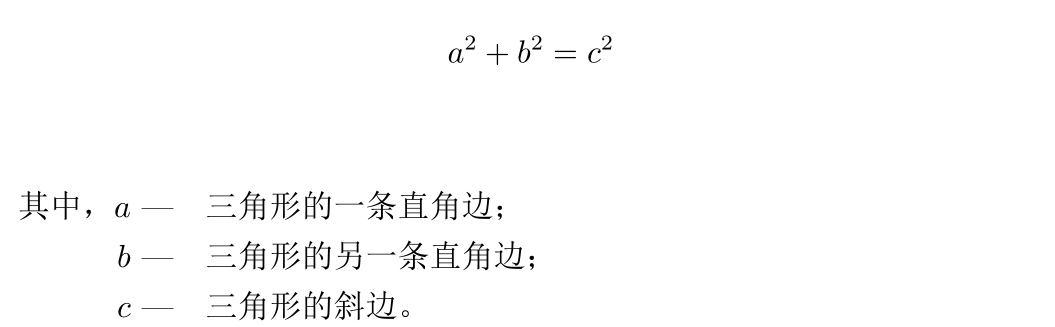
\includegraphics[width=0.8\linewidth]{include/images/hang}}}


\faq{行内公式的情况下如何让sum prod这些运算符的上下标在头上和脚下?}{}

这样处理行内公式的上下标会导致段落行距不整齐,不符合 \LaTeX{}
的审美。如果彻底放弃审美,可以使用 \cs{limits} 命令,如:

%\begin{verbatim}
\begin{example}
$\sum\limits_{i=1}^n, \prod\limits_\epsilon$
\end{example}
%\end{verbatim}

%效果是这样的:$\sum\limits_{i=1}^n \quad \prod\limits_\epsilon$

\faq{如何将积分的上限标放在积分号的上下两侧?}{}

积分号的上下限放置在积分号的右侧是英美国家和 \LaTeX{}
的排版习惯,通常无需处理。
如果你很确定需要按照 ISO 80000-2:2009 或者 GB 3102.11-93 的规定排版积分号,可以:

\begin{enumerate}
\def\labelenumi{\arabic{enumi}.}

\item
  在调用 amsmath 宏包时添加 intlimits 选项;
\item
  \texttt{\cs{def}\cs{int}\{\cs{intop}\}}
\item
  如果使用 unicode-math 宏包,
\end{enumerate}

\begin{texlist}
\removenolimits{%
  \int\iint\iiint\iiiint\oint\oiint\oiiint
  \intclockwise\varointclockwise\ointctrclockwise\sumint
  \intbar\intBar\fint\cirfnint\awint\rppolint
  \scpolint\npolint\pointint\sqint\intlarhk\intx
  \intcap\intcup\upint\lowint
}
\end{texlist}


\faq{如何自定义数学运算符,然后让下标放在脚下?}{}

借助 amsmath 包(实际上是amsmath自动调用的amsopn宏包)的
\cs{DeclareMathOperator*} 命令,可以在导言区定义需要的数学运算符(需要注意加不加*是有区别的)。例如

\begin{texlist}
\DeclareMathOperator*{\esssup}{ess\,sup}
\end{texlist}

\begin{example}
\[ 
  \esssup_{x\in {R}} 
\]
\end{example}


对于只是偶尔用到的运算符,也可以无需定义而直接在数学模式中使用新算符定义命令。
%
%例如
%|\operatorname*{ess\,sup}_{x\in {R}}|

\begin{example}
\[
  \operatorname*{ess\,sup}_{x\in {R}}
\]
\end{example}


\faq{行列式变换过程中,我们一般是在中间的箭头上表示出变换的方式,如何才能在长箭头上打出多行内容?}{}
可以看看amsmath宏包提供的长箭头命令。
\begin{example}
\[
  A \xleftarrow[formula-1]{formula-2} B,
  C \xrightarrow[formula-1]{formula-2} D
\]

\end{example}

\faq{如何输出反斜杠?}{}
方式很多,例如
\begin{example}
  \textbackslash \quad 或者 \quad \verb|\|
\end{example}
%
%\begin{texlist}
%    \textbackslash 或者 \verb|\|
%\end{texlist}


\faq{对equation环境下的公式、图片编号按章节、小节进行重新定义}{}

公式编号使用amsmath宏包的numberwithin设定关联即可。
图片编号可以使用caption宏包自定义格式。

\faq{带括号的公式有哪些折行方式?在括号中间折行。}{}
使用| \left( \right) |括起来的内容不能直接折行,但是可以变通,比如使用| \left( | 匹配 | \right. | 和 | \left. | 匹配 | \right) |,
这时候需要借助幻影、支柱等方法处理各行内容高度不同带来的括号大小不同问题。

\faq{怎么在极限符号下面打出x→0 }{}
很简单的基本指令就行,例如|\lim\limits_{x \to 0}|得到$\lim\limits_{x \to 0}$
\begin{example}
\[
  \lim\limits_{x \to 0}
\]
\end{example}

\faq{\LaTeX{}敲的公式可以插入word吗?}{}
可以,但是不推荐。

\faq{公式中的文本怎么输入?}{}
公式中的文本输入,可以用 \verb|\mbox{...}|。使用率较高的是 \texttt{amstext} 宏包中提供了\verb|\text|命令,示例如下:
\begin{example}
\begin{center}
  This is $_{\text{subscript}}$\\
  This is $_{\mbox{subscript}}$
\end{center}
\[a = b, \text{\qquad by assumption}\]
\end{example}

%\begin{note}\small \itshape
	我们加载 amsmath 宏包的时候,系统会自动调用amstext, amsbsy, amsopn,
	amsintx包,所以无需我们额外加载包。
%\end{note}
%\begin{note}
%	\small \itshape

 这里需要注意的是若是我们的文本部分与其他字符有间隔,需要在\verb|\text{}|里面进行添加。
%\end{note}
%\fancybreak
\faq{如何输入连分数?}{}
\verb|amsmath| 宏包提供的命令 \verb|cfrac| 用于排版连分数,比我们直接使用 \verb|\frac| 排版的效果要好。如:
\begin{example}
\[
  \cfrac{1}{\sqrt 2 + \cfrac{1}{\sqrt 2 +\dotsb}},\quad
  \frac{1}{\sqrt 2 + \frac{1}{\sqrt 2 +\dotsb}}
\]
\end{example}


\faq{如何输入带方框的公式?}{}


可以使用命令 \verb|boxed| 将公式放在方框中,这个命令类似 \verb|\fbox| 如
\begin{example}
\[
  \boxed{\eta \leq C \text{ and } C \leq \Delta}
\]
\end{example}

另外,\verb|fancybox| 宏包提供的几个环境和命令会把公式的编号和公式一起放在方框中。

\faq{实数域 $\mathbb{R}$ 或复数域 $\mathbb{C}$ 等的字体该用什么命令?}{}
使用 amsfonts 宏包提供的\verb|\mathbb{字母}|命令, 例如:
\begin{example}
 $x \in \mathbb{R}$ and $c \in \mathbb{C}$
\end{example}



通常,排版时有些符号需要特殊字体,这里简单列举常用的几个字体。

%\begin{center}
%\includegraphics{fig2}
%\end{center}

{\small\begin{tabular}{ll}
		\hline
		命令&样例\\
		\hline
		默认&${ABCDEFGHIJKLMNOPQRSTUV WXYZ}$\\
		&${abcdefghijklmnopqrstuvwxyz}$\\
		\verb|\mathit|&$\mathit{ABCDEFGHIJKLMNOPQRSTUV WXYZ}$\\
		&$\mathit{abcdefghijklmnopqrstuvwxyz}$\\
		\verb|\mathbf|&$\mathbf{ABCDEFGHIJKLMNOPQRSTUV WXYZ}$\\
		&$\mathbf{abcdefghijklmnopqrstuvwxyz}$\\
		\verb|\mathrm|&$\mathrm{ABCDEFGHIJKLMNOPQRSTUV WXYZ}$\\
		&$\mathrm{abcdefghijklmnopqrstuvwxyz}$\\
		\verb|\mathsf|&\textsf{ABCDEFGHIJKLMNOPQRSTUV WXYZ}\\
		&\textsf{abcdefghijklmnopqrstuvwxyz}\\
%        |\bm|$^a$ & $\bm{ABCDEFGHIJKLMNOPQRSTUV WXYZ}$\\
%        & $\bm{abcdefghijklmnopqrstuvwxyz}$\\
		\verb|\mathscr|$^a$&{\usefont{U}{rsfs}{m}{n}ABCDEFGHIJKLMNOPQRSTUV WXYZ}\\
		\verb|\mathfrak|$^b$&{\fontencoding{U}\fontfamily{euf}\selectfont ABCDEFGHIJKLMNOPQRSTUV WXYZ}\\
		&{\fontencoding{U}\fontfamily{euf}\selectfont abcdefghijklmnopqrstuvwxyz}\\
		\verb|\mathcal|&$\mathcal{ABCDEFGHIJKLMNOPQRSTUV WXYZ}$\\
		\verb|\mathbb|$^c$&$\mathbb{ABCDEFGHIJKLMNOPQRSTUV WXYZ}$\\
		\hline
%		$^a$ 需要 \verb|bm|宏包&\\
		$^a$ 需要 \verb|mathrsfs|宏包&\\$^b$ 需要 \verb|amsfonts|宏包&\\$^c$ 需要 \verb|amsfonts|宏包&\\
\end{tabular}}

\faq{$n$次根式 $\sqrt[n]{\text{Roots}}$ 的位置调整}{}
通常,我们用 \verb|\sqrt[...]{...}| 来输入公式。
\begin{example}
$\sqrt2$, $\sqrt2y$, $\sqrt{2y}$\\
$\sqrt[3]{2}$, $\sqrt[n+1]{x+y}$
\end{example}

按照如上的输入方式,我们输入如下公式 \verb|$\sqrt[\frac{1}{n}]{a}$| 会输出 $\sqrt[\frac{1}{n}]{a}$ ,而 \verb|$\sqrt[\beta]{a}$| 输出为 $\sqrt[\beta]{a}$。
我们需要这样调整:
\begin{example}
$\sqrt[\leftroot{2}\uproot{4}\beta]{k}$,
$\sqrt[\leftroot{1}\uproot{3}\beta]{k}$,
$\sqrt[\leftroot{2}\uproot{4}\frac{1}{n}]{k}$,
$\sqrt[\leftroot{1}\uproot{3}\frac{1}{n}]{k}$
\end{example}
\noindent 这两个命令 \verb|leftroot| 和 \verb|uproot| 分别表示将方根向左向上移动 $n$ 个单位,若为负数表示向反方向移动。


\faq{如何输入在等号上输入如 def 等文字?}{}

对于这种特殊的重叠符号,可通过使用 \verb|amsmath| 宏包的 \verb|overset|
命令来实现。具体用法见下面的例子。
\begin{example}
\begin{equation}a\overset{?}{=}b\end{equation}
\end{example}

若等号上文字较多时,这时我们可以用 \verb|extarrows| 宏包的自适应长度的等号,简单示例如下:
\begin{example}
\begin{equation}
  a\xlongequal[abc]{def}b
\end{equation}
\end{example}

\faq{公式中大写希腊字母怎么改成粗斜体?}{}
希腊字母大写均为正体,若需要改成斜体,用下面的命令就好:
\begin{example}
$\Gamma$, $\varGamma$. $\Delta$, $\varDelta$.
$\Theta$, $\varTheta$. $\Lambda$, $\varLambda$.
$\Xi$, $\varXi$, $\Sigma$,  $\varSigma$.
$\Upsilon$, $\varUpsilon$. $\Phi$, $\varPhi$.
$\Psi$, $\varPsi$.
\end{example}

\faq{公式中小写希腊字母怎么改成正体?}{}

使用 \verb|upgreek| 包提供的直立的希腊字母,这里简单列举部分符号如下:
\begin{center}
	\begin{tabular}{*4{ll}}
		\K{\upalpha}      & \K{\uptheta}      & \K{\uppi}         & \K{\upphi}        \\
		\K{\upbeta}       & \K{\upvartheta}   & \K{\upvarpi}      & \K{\upvarphi}     \\
		\K{\upgamma }     & \K{\upiota}       & \K{\uprho}        & \K{\upchi}        \\
		\K{\updelta}      & \K{\upkappa}      & \K{\upvarrho}     & \K{\uppsi}        \\
		%\K{\upepsilon}    & \K{\uplambda}     & \K{\upsigma}      & \K{\upomega}      \\
		%\K{\upvarepsilon} & \K{\upmu}         & \K{\upvarsigma}                     \\
		%\K{\upzeta}       & \K{\upnu}         & \K{\uptau}                          \\
		%\K{\upeta}        & \K{\upxi}         & \K{\upupsilon}                      \\
		%                                                                      \\
		%\K\Upgamma      & \K\Uplambda     & \K\Upsigma      & \K\Uppsi        \\
		%\K\Updelta      & \K\Upxi         & \K\Upupsilon    & \K\Upomega      \\
		%\K\Uptheta      & \K\Uppi         & \K\Upphi                          \\
	\end{tabular}
\end{center}

\faq{如何输入数学公式里面的矢量?}{}


\fbox{第一种方法},使用 \verb|harpoon| 宏包,
\begin{texlist}
\overrightharp{this}
\end{texlist}



\fbox{第二种方法},
自己定义一个命令。如下:
%\begin{Verbatim}[frame=single,rulecolor=\color{niceblue},fontsize=\small]
%\newcommand{\myvec}[1]%
%  {\stackrel{\raisebox{-2pt}[0pt][0pt]{\small$\rightharpoonup$}}{#1}}
%\end{Verbatim}
\begin{texlist}
\newcommand{\myvec}[1]%
{\stackrel{\raisebox{-2pt}[0pt][0pt]
		{\small$\rightharpoonup$}}{#1}}
\[
	\myvec{A}
\]
\end{texlist}

\faq{常见矩阵的输入方法。}{}
我们经常会见到如下矩阵:
\begin{example}
\begin{gather*}
 \begin{matrix}  0 &  1 \\ 1 &  0 \end{matrix}\quad
 \begin{pmatrix} 0 & -i \\ i &  0 \end{pmatrix}\\
 \begin{bmatrix} 0 & -1 \\ 1 &  0 \end{bmatrix}\quad
 \begin{Bmatrix} 1 &  0 \\ 0 & -1 \end{Bmatrix}\\
 \begin{vmatrix} a &  b \\ c &  d \end{vmatrix}\quad
 \begin{Vmatrix} i &  0 \\ 0 & -i \end{Vmatrix}
\end{gather*}
\end{example}

很多用户刚开始的时候用 \verb|array| 环境来输入矩阵,示例如下:
\begin{example}
\begin{gather*}
 \begin{array}{cc}  0 &  1 \\ 1 &  0 \end{array}  \quad
 \left(\begin{array}{cc}  0 & -i \\ i &  0 \end{array}\right) \\
 \left[\begin{array}{cc} 0 & -1 \\ 1 &  0 \end{array}\right] \quad
 \left\{\begin{array}{cc} 1 &  0 \\ 0 & -1 \end{array}\right\} \\
 \left|\begin{array}{cc} a &  b \\ c &  d \end{array}\right| \quad
 \left\|\begin{array}{cc} i &  0 \\ 0 & -i \end{array}\right\|
\end{gather*}
\end{example}

当然,大家可比较两个输出结果,择其一使用。

\faq{如何输入三角矩阵,常见的 $n$ 阶矩阵?}{}
这个问题我们提供一些实例,也可以用其他方法来写,实例选自``\LaTeX{}入门与提高'',另外,我们需要读读
amsmath输入矩阵的常用的方法,有 \verb|array| 环境、\verb|matrix| 环境、\verb|bmatrix| 环境、\verb|pmatrix| 环境等。
\begin{example}
\[\left(\begin{array}{cccc}
  a_{11} & a_{12} & \cdots & a_{1n} \\
  &a_{22}  & \cdots &a_{2n}  \\
  &        & \ddots & \vdots \\
  \multicolumn{2}{c}{\raisebox{1.3ex}[0pt]{\Huge0}}
  &        &a_{nn}
\end{array}\right)\]
\[\begin{pmatrix}
  a_{11} & a_{12} & \cdots & a_{1n} \\
  &a_{22}  & \cdots &a_{2n}  \\
  &        & \ddots & \vdots \\
  \multicolumn{2}{c}{\raisebox{1.3ex}[0pt]{\Huge0}}
  &        &a_{nn}
\end{pmatrix}\]
\end{example}
\begin{example}
\[
 \begin{array}{c@{\hspace{-5pt}}l}
  \left(\begin{array}{ccc|ccc}
   a&\cdots &a &b &\cdots&b\\
   &\ddots &\vdots &\vdots &\adots\\
   & &a& b \\\hline
   & & & c &\cdots &c\\
   & & & \vdots& &\vdots\\
   \multicolumn{3}{c|}{\raisebox{2ex}[0pt]{\Huge0}}
   & c & \cdots & c
  \end{array}\right)
  &\begin{array}{l}
    \left.\rule{0mm}{7mm}\right\}p\\
	\\\left.\rule{0mm}{7mm}\right\}q
   \end{array}\\[-5pt]
  \begin{array}{cc}
   \underbrace{\rule{17mm}{0mm}}_m&
   \underbrace{\rule{17mm}{0mm}}_m
  \end{array}&
 \end{array}
\]
\end{example}
\begin{example}
\[
 \begin{pmatrix}
  a_{11}&a_{12}&\ldots&a_{1n}\\
  a_{21}&a_{22}&\ldots&a_{2n}\\
  \hdotsfor{4}\\
  a_{n1}&a_{n2}&\ldots&a_{nn}\\
 \end{pmatrix}
\]
和
\[
 \begin{pmatrix}
  a_{11}&a_{12}&\ldots&a_{1n}\\
  a_{21}&a_{22}&\ldots&a_{2n}\\
  \vdots &\vdots &    &\vdots\\
  a_{n1}&a_{n2}&\ldots&a_{nn}\\
 \end{pmatrix}
\]
\end{example}

\fancybreak \faq{如何把行间的矩阵缩小一点?}{}
\LaTeX{}处理公式非常漂亮,但是遇到行间的矩阵,往往会扩大我们的行间距来满足矩阵的显示空间,这样整体不是
很美观,而且也会出现溢出或者段落调整带来的诸多问题。这里面的行间矩阵是这样处理的,需要用到 amsmath 包提供的 \verb|smallmatrix| 环境即可。

请看下面效果:
\begin{example}
To show the effect of the matrix on surrounding
lines inside a paragraph, we put it here:
$\begin{pmatrix}\begin{smallmatrix}
	1 & 0 \\
	0 & -1
\end{smallmatrix}\end{pmatrix}$
and follow it with enough text to ensure that
there is at least one full line below the matrix.
\end{example}

上面的方法也适合于行间公式,即当我们的矩阵过大引起了行溢出,可以用这一环境来进行瘦身。



\fancybreak \faq{带有上下括号的公式怎么排?}{}
通常我们会遇到一些公式,需要用大括号对其进行注释说明,这类公式虽然遇到不多,但是也非常实用。
我们看下面的例子

\begin{example}
\[
 \underbrace{a + \overbrace{b+\cdots}^{{}=t}+z}
	_{\text{total}} ~~ 
 a + {\overbrace{b+\cdots}}^{126}+z
\]
\end{example}

\begin{note}\small \itshape
	这里需要注意的是前后两个括号的上标位置不同,大家要细看其上标使用的方法。若是上标紧跟\verb|\overbrace{}|那么上标会在其上方或者下方的居中位置,其他情况,参看上面实例。
\end{note}



\fancybreak \faq{如何手动编号, {\ttfamily\textbackslash[...\textbackslash]} 与{\ttfamily \$\$...\$\$} 有什么差异?}{}

\jieshi

我们知道,行间公式(display)有两种情况,一类带编号,另一类不带编号。故而,我们常用 \verb|equation| 环境来输入行间公式可以自动编号。如
\begin{example}
\begin{equation}
	a^2 + b^2 = c^2.
\end{equation}
\end{example}
\noindent 而不带编号的行间公式则使用 \verb|\[..\]| 或 \verb|displaymath|的环境来输入的。如
\begin{example}
\[
 a^2 + b^2 = c^2.
\]
\begin{displaymath}
 a^2 + b^2 = c^2.
\end{displaymath}
\end{example}

\jiejue

若是需要手动编号,只需使用 \verb|\eqno| 或 \verb|\leqno| ,一个编号是在右边,一个编号在左边,如下实例:
\begin{example}
\[
 a^2 + b^2 = c^2.\eqno{(1)}
\]
\begin{displaymath}
 a^2 + b^2 = c^2.\leqno{(3)}
\end{displaymath}
\end{example}

这里简要说明下\verb|\[...\]|与\verb|$$...$$|的差异。\verb|$$...$$|是 Plain \TeX{}的命令。它会修改公式的垂直间距,而使得全文的公式间距不一致。我们在使用 \LaTeX{}
的时候,应避免使用\verb|$$...$$|,最为重要的是:
当我们使用 amsmath 宏包的公式居左参数fleqn加上的时候,使用\verb|$$...$$|输入的公式是不能左对齐的,参看``An essential guide to \LaTeXe{} usage\footnote{\url{ftp://ftp.tex.ac.uk/tex-archive/info/l2tabu/english/l2tabuen.pdf}}'' 及 ``\href{http://www.tex.ac.uk/cgi-bin/texfaq2html?label=dolldoll}{Why use \textbackslash [...\textbackslash ] in place of \$\$...\$\$}''。



\fancybreak

\faq{怎样改变\LaTeX{}公式字体的大小?}{}

在数学模式中,有四个控制字体相对大小的命令,即

\begin{center}
	\begin{tabular}{lcl}
		\verb|\displaystyle|& D &行间公式的基本尺寸\\
		\verb|\textstyle| & T & 行内公式的基本尺寸大小\\
		\verb|\scriptstyle| & S & 一级角标的尺寸\\
		\verb|\scriptscirptstyle| & SS & 二级角标的尺寸大小\\
	\end{tabular}
\end{center}

\jiejue

上述命令如何使用,我们输入这样的一个公式
\begin{example}
一个行内分式 $\frac{1}{a + b}$.
\end{example}
\noindent 我们想要分式能显示得更为清晰些。我们可以用
\begin{example}
一个行内分式 $\displaystyle\frac{1}{a + b}$.
\end{example}
\noindent 这也是行内公式显示为行间公式的方法,您可以尝试其他命令来实践一下效果。


我们能否像修改正文字体那样来修改公式字体呢?回答是肯定的。

\begin{example}
\begin{small}
\begin{equation}
	A \times B = C
\end{equation}
\end{small}
\end{example}

当然,如果是想批量更改的话,最好定义新的环境:
\begin{texlist}
\newenvironment{sequation}{\small\begin{equation}}{\end{equation}}
\newenvironment{tequation}{\tiny\begin{equation}}{\end{equation}}
\end{texlist}
\newenvironment{sequation}{\small\begin{equation}}{\end{equation}}
\newenvironment{tequation}{\tiny\begin{equation}}{\end{equation}}
\begin{example}
\begin{tequation}
	A \times B = C
\end{tequation}
\end{example}

\jieshi

更为高级的设置方式如下:

\LaTeX{}根据文本字体的大小,调整公式的大小。
通常我们不必做什么修改,当然也可以自己定义,用到的命令为 
\begin{texlist}
\DeclareMathSizes{ds}{ts}{ss}{sss}
\end{texlist}
\noindent 分别对应\verb|displaystyle|,\verb|textstyle|,\verb|scriptstyle|,\verb|scriptscirptstyle|的尺寸。


例如,下面一段代码加在文档 ``preamable'' 部分就可以实现对公式大小的修改:

\begin{texlist}
% Size of the math equations
\DeclareMathSizes{10}{10}{7}{5}
\DeclareMathSizes{11}{11}{7.7}{5.5}
\DeclareMathSizes{12}{12}{8.4}{6}
\DeclareMathSizes{13}{13}{9.1}{6.5}
\DeclareMathSizes{14}{14}{9.8}{7}
\end{texlist}
上面,第一个大括号里是文档使用的字号。只有在这与文档中字号定义相同时,后面对于公式
大小的定义才有效。后面三个大括号分别定义的是,普通公式字号、第一级上下标、第二级上下标的字号大小。


如果在一个使用12号字体的文档里,使用
\begin{texlist}
\DeclareMathSizes{12}{20}{14}{10}
\end{texlist}
就可以得到,相对大的公式。
\begin{note}
	上文中,我们用 \verb|\displaystyle| 来使得行内分式变成行间分式大小,实际上,amsmath宏包提供了一个命令 \verb|\dfrac|,我常称``大分式'',而 \verb|textstyle| 对应的命令为 \verb|\tfrac|。我们看如下示例:
\begin{example}
$-2<\dfrac{1}{x+1}$ \quad
$-2<\tfrac{1}{x+1}$
\end{example}
\end{note}

\fancybreak


\faq{如何使上下限出现在求和、 积分符号的上下方而不是右边?}{}
数学公式中求和、积分符号的上下限的位置取决于是行内公式(inline)还是特显公式(display)\footnote{由于中文资料的翻译不同,我这里统一称行内公式(inline)和行间公式(display)。}。在行内公式中,其上下限出现在符号的右边,
而在独立公式中出现在符号的上下方。前者是指在正文插
入和文字混同的数学公式,后者独立一行排版,可以有或没有编号。

例如:

\begin{example}
首先,我们看看行内公式的显示
 $\sum_{i = 1}^n a_i$
 其对应的行间公式如下:
\[
 \sum_{i = 1}^n a_i
\]
积分示例如:$\int_0^R \frac{2x\,dx}{1+x^2}$,
行间公式如:
\[
 \int_0^R \frac{2x\,dx}{1+x^2}
\]
\end{example}

这里我们注意到,在行间公式和独立公式中求和号的上下限是不同的,而积分号则相同。一般情况下我们用默认即可,因为\TeX{} 为了让我们的版面整体排版美观做了这样的差异处理。有时,我们用户有特殊需要,想自己调整其显示位置,我们就如下方法。

\fbox{第一种方法},需要用到 \verb|\limits| 和 \verb|nolimits| 这两个命令。

具体代码实现如下:
\begin{example}
我们看看这个效果$\sum\limits_{i = 1}^n a_i$ 和
\[
 \sum\nolimits_{i = 1}^n a_i 
\]
\end{example}

这样我们就把这二者样式对调过来了,即在行间显示特显模式,在特显模式下显示行间模式。实际我们可以这样认为,limits 的英文有限制约束的含义,我们用这个命令就是要把不受控制的下标限制到求和号上下的位置。这样我们对于积分有:
\begin{example}
\[
 \int\limits_0^R \frac{2x\,dx}{1+x^2}
\]
\end{example}

\fbox{第二种方法},如果我们的公式较多,上面的方法的确太过繁琐,有没有一劳永逸的方案,这里给大家补充我们平时不很注意的知识。
amsmath 宏包加载的时候,我们可以设置某些参数来实现其对应的功能。

amsmath 与上下标有关的参数介绍如下:

\begin{description}
	\item[sumlimits] 该选项为缺省值,其功能是将求和号($\sum$)、连乘号($\prod$)等符号(除积分号外)的上下标按照如下规则来排版:
	若这类符号出现在单独排列的数学环境中,则其上下标将分别排印在这类符号的上面和下面居中的位置上;若这类符号
	出现在文中混排的数学环境里,则其上下标将分别排在这类符号的右上角和左下角的位置。
	\item[nosumlimits] 该选项的功能是,不论求和号、连乘号等符号(除积分号外)的上下标总是将其上下标将分别排在这类符号的右上角和左下角的位置。
	\item[intlimits]该选项仅对积分号($\int$等)而言,其功能与选项 sumlimits 的功能完全一致。
	\item[nointlimits]该选项为缺省值,其功能为:不论积分号是否出现在何种数学环境中,其上下标总是排印在积分号的
	左上角和右下角与之平齐的位置上。
	\item[namelimits]该选项为缺省值,其功能与选项 sumlimits 基本一致,只是该选项针对的是 $\det$, $\inf$, $\lim$, $\max$, $\min$ 等一些带有下标的函数名而言的。
	\item[nonamelimits]该选项的功能是,不论上面所述的函数名在何种数学环境里,其下标总是排在函数名右下角与之平齐
	的位置上。
\end{description}
这个包的其他参数如\verb|leqno|, \verb|fleqn| 等等,我们这里不再多述,后续问题会有简单涉及。

\begin{note}\small 
	amsmath宏包的参数的含义搞清晰了,我们就可以自己指定其上下标位置了。实际上,上面的参数也不是万能的,大家
	细细研读就会明白,有些效果还是实现不来,只能手工处理。
\end{note}

\fancybreak
\faq{如何输入组合数?}{}
较为常用的命令是 \verb|amsmath| 提供的 `\verb|\binom{...}{...}|'。如:
\begin{example}
In inline mode: $\binom{k}{2}$.\\
In display mode:
\begin{displaymath}
 \binom{k}{2}
\end{displaymath}
\end{example}

这里有个问题是 \verb|\binom| 命令会在行间模式和行内模式变换自己的个头,
若是需要随意改换其个头,可以使用 \verb|\tbinom| 和 \verb|dbinom|。例如:
\begin{example}
In inline mode: $\dbinom{k}{2}$,
which is horrible.\\
In display mode:
\begin{equation*}
 \tbinom{k}{2}.
\end{equation*}
\end{example}


\fancybreak \faq{如何排版公式的多行下标?}{}
多行下标或者上标较为实用的技巧,我们可以使用命令 \verb|\substack|,这条命令的上标或者下标均是中心对齐的。

更为一般的情况是,使用 \verb|subarray|环境来实现多行上下标,且可以自己选择对齐方式。

\begin{example}
\begin{gather}
 \sum_{\substack{0 \le i \le m\\
	0 < j < n}}P(i, j)\\
 \sum_{\begin{subarray}{l}
	i \in \Lambda   \\
	0 \le i \le m   \\
	0 < j < n
	\end{subarray}} P(i, j)
\end{gather}
\end{example}
\noindent \verb|subarray| 的选项 \verb|l| 代表左对齐,也可换为 \verb|c|,\verb|r|分别代表
中心对齐和右对齐。

\fancybreak \faq{怎样增加斜杠分数线的长度?}{}

我们输入行内分数或者在较复杂的公式中,常常用 \verb|/|来作为分数线。如 \verb|$1/2$| 得到 $1/2$。
当我们的分子或分母出现大符号时,如 $\sum_1^n a_i /2$ ,我们发现分数线不够美观,也不会随着分数线左右内容的变化而变化,有时会影响到公式含义
的表达。有网友问及,如何定义一个可以伸缩的斜线,如下的两个方法可以解决大家的问题。

\jiejue

\begin{enumerate}%[(1)]
	\item 我们可以使用宏包 \verb|nicefrac|来实现我们想要的结果,用在数学模式中,主要用在行内公式中,如
\begin{example}
 $\nicefrac{1}{2}$
\end{example}
	\noindent 若是我们把它用在行间公式中,结果
\begin{example}
\[
 \nicefrac{\sum_1^n a_i}{2}
\]
\end{example}
	\item 上面的方法常用于简单的行内分式输入,这里介绍一个更为通用的方法如下:
\begin{example}
\[
 \left. \sum_1^n a_i \middle/ 2 \right.
\]
\end{example}
	\noindent 也可自己用定界符的大小控制来调节。
\begin{example}
\[
 \sum_1^n a_i \Biggm/ 2 
\]
\end{example}
\end{enumerate}

\begin{note}
	\verb|nicefrac| 宏包也可以指定分式所用的字体,也可用在非数学模式中如
\begin{example}
 \nicefrac[\texttt]{1}{2}\\
 \nicefrac[\texttt]{\textit{1}}{2}\\
 $\nicefrac[\mathcal]{A}{B}$
\end{example}
	\noindent 其衍生宏包 \verb|units| 可用于输入物理单位,示例:
\begin{texlist}
 \sffamily\bfseries\unit{m}\\
 \sffamily\bfseries$\unit{m}$\\
 \sffamily\itshape\unit[1]{m}\\
 \sffamily\itshape$\unit[1]{m}$\\
 \sffamily\bfseries\unitfrac{m}{s}\\
 \sffamily\bfseries$\unitfrac{m}{s}$
\end{texlist}
\end{note}
\fancybreak \faq{如何让公式编号与章节关联?}{}

\jieyong{初级做法}

有用户使用下面的方式来添加公式与章节关联,
\begin{texlist}
\renewcommand{\theequation}{\arabic{section}.\arabic{equation}}
\end{texlist}
\noindent 这一做法有个不好的地方就是:当\verb|section| 计数器增加时, \verb|equation| 计数器不会自动置零。

解决这一问题导言区需要加上如下代码:
\begin{texlist}
\makeatletter
 \@addtoreset{equation}{section}
\makeatother
\end{texlist}
\noindent 或者每次使用 \verb|section| 命令之后,把 \verb|equation| 的计数器设置为 0。


\jiejue

通常,可使用 amsmath 宏包提供的 \verb|numberwithin| 命令来实现与章节的关联,即
\begin{texlist}
\numberwithin{equation}{section}
\end{texlist}

\noindent 每次当 \verb|section| 计数器加1时,\verb|equation| 会自动置零。
这样就可以方便地实现公式编号与章节之间的关联了。


\fancybreak \faq{如何输入分段函数?}{}

分段函数的输入方法很多,这里给大家介绍下:

\fbox{第一种方法},使用 \verb|amsmath| 包提供的 \verb|cases| 环境

\begin{example}
\[
 P_{r,j}=\begin{cases}
  0 & \text{$r-j$ 为奇数},\\
  r!\,(-1)^{(r-j)/2} &
  \text{$r-j$ 为偶数}.
 \end{cases}
\]
\end{example}

\fbox{第二种方法},使用 \verb|array| 环境,实例如下:
\begin{example}
\[
 P_{r,j}=\left\{\begin{array}{ll}
  0 & \text{$r-j$ 为奇数},\\
  r!\,(-1)^{(r-j)/2} &
  \text{$r-j$ 为偶数}.
 \end{array}\right.
\]
\end{example}



\fbox{第三种方法},使用 \verb|aligned|环境,示例如下:
\begin{example}
\begin{equation*}
 \left.\begin{aligned}
  B' & =-\partial\times E,\\
  E' & =\partial\times B - 4\pi j,
 \end{aligned}\right\}
  \quad \text{Maxwell方程}
\end{equation*}
\end{example}


\fancybreak \faq{多行公式中如何换页?}{}

\jieyong{问题描述}

输入带有较多公式的文章时,经常遇到如下情况:当一页余下的空间不足以安置公式时,若公式为单行公式看着不很明显,
若是多行公式,会发现当前页会产生较多空白,这时该怎么办?


\jiejue

在导言区加入
\begin{texlist}
\usepackage{amsmath}
\allowdisplaybreaks[4]
\end{texlist}

\jieshi

由于公式默认是不允许跨页显示的,如果有较长的公式,则公式可能就需要跨页显示。
命令 \verb|\allowdisplaybreaks| 后面还有个选项\verb|[n]|,其完整形式是\verb|\allowdisplaybreaks[n]|,
其中 \verb|n| 是1-4之间的数,
表示允许换页的程度,如\verb|\allowdisplaybreaks[0]|表示可以换页
但尽量不换,而\verb|\allowdisplaybreaks[4]|则是强制换页等同于
\verb|\allowdisplaybreaks|。注意上述命令放在导言区使用。

另外,也可以不在导言区使用\verb|\allowdisplaybreaks|,在想换页处使用 \verb|\displaybreak|,它也带有选项[n], 意义与前面的相同,该命令最好放在换行符\verb|\\|之前。
我们也可以在多行公式的行之间使用\verb|\\*|
来阻止此处换行。

\begin{note}
	需要注意的是:有些多行公式环境是将内容放在一个不可分割的盒子中的,因此在这样的环境中 命令 \verb|\displaybreak| 和 \verb|\allowdisplaybreaks|都是不起作用的。这些环境包括
	\verb|split|,\verb|aligned|,\verb|gathered|和 \verb|alignedat|。
\end{note}

\fancybreak

\faq{数学常用环境的中文化}{}
可以使用如下代码来处理。
\begin{texlist}
\newtheorem{theorem}{{定理}}
\newtheorem{proposition}{{命题}}
\newtheorem{lemma}{{引理}}
\newtheorem{corollary}{{推论}}[theorem]
\newtheorem{definition}{{定义}}
\newtheorem{example}{{例}}
\end{texlist}

有时,我们想要定理,定义等有一个缩进,可以使用 \verb|ntheorem| 宏包来定义其格式。较为顺手使用的可以用如下
定义:
\begin{texlist}
\newtheorem{theorem}{\hskip 2em{定理}}
\newtheorem{proposition}{\hskip 2em{命题}}
\newtheorem{lemma}{\hskip 2em{引理}}
\newtheorem{corollary}{\hskip 2em{推论}}[theorem]
\newtheorem{definition}{\hskip 2em{定义}}
\newtheorem{texlist}{\hskip 2em{例}}
\end{texlist}

\faq{如何实现公式的引用(括号引用) ?}{}

在引用公式的时候,通常要给公式编号加上括号,一般的 \verb|ref| 命令可实
现公式的引用, 但无括号, 而 \verb|eqref| 则可达到上述效果的公式引用。如
\begin{example}
\begin{equation}
 a = b - 1\label{eq:test}
\end{equation}
由公式 \eqref{eq:test}, 可得...。
\end{example}
\hfill ---选自《My-FAQ》



\fancybreak \faq{如何在公式中添加脚注?}{}

一般公式,我们可以用 \verb|footnote| 命令,有些环境不可使用,可以用 \verb|footnotemark| 和 \verb|footnotetext| 命令来实现。如下:
\begin{example}
\renewcommand{\thefootnote}{{\arabic{footnote}}}
\begin{minipage}{.8\textwidth}
\begin{equation}
  a^2 + b^2 = c^2 \footnote{勾股定理}
\end{equation}
\begin{align}
  X = \sum_{1\le i\le j\le n} X_{ij}
   \footnotemark[2]
\end{align}
\footnotetext[2]{align里的footnote}
\end{minipage}
\end{example}





\fancybreak \faq{如何让一公式编号表示为另一公式编号的变化形式?}{}


我们经常使用一个公式编号加上某些符号如一撇 来表示公式的一个变化。这样的公式编号可以通过\texttt{amsmath}宏包的\verb|\tag|命令加上\LaTeX{}的引用机制来实现。例如:
\begin{example}
\begin{equation} \label{eq:original}
  A = B
\end{equation}
\begin{equation}
\tag{\ref{eq:original}$'$} \label{eq:origprime}
  A = B + 1
\end{equation}
\end{example}
\hfill ---选自《CTeX-FAQ》

\fancybreak \faq{如何断行括号内的长公式?}{}
\jieyong{通常做法}
因为自适应定界符 \verb|\left\{| \verb|\right\}|中间不能断行,所以我们通常的做法有如下几个:

\begin{example}
\begin{equation}
\begin{split}
 a = &\left\{c + d + e + f + g + h +l
  + m\rule{0pt}{15pt}\right.\\
 &\left.\rule{0pt}{15pt}+ \sqrt{f + g + h}
  + \sum_{i=1}^n a_i \right\}\\
 &+ n + o
\end{split}
\end{equation}
\begin{equation}
\begin{split}
 a = &\left\{c + d + e + f + g + h +l
  + m\vphantom{\sum_{i=1}^n a_i}\right.\\
 &\left.\vphantom{\sum_{i=1}^n a_i}+
  \sqrt{f + g + h}+\sum_{i=1}^n a_i\right\}\\
 &+ n + o
\end{split}
\end{equation}
\begin{equation}
\begin{split}
 a = &\Biggl\{c + d + e + f + g + h +l
  + m\vphantom{\sum_{i=1}^n a_i}\\
 & +   \sqrt{f + g + h} +
  \sum_{i=1}^n a_i \Biggr\} \\
 &+ n + o
\end{split}
\end{equation}
\end{example}
如上方法中,均需要我们做些额外的工作,能否保留下自适应定界符 \verb|\left\{| \verb|\right\}| 系统自动断行呢?

%这里我们推荐下 \verb|breqn| 宏包\footnote{\url{http://www.ctan.org/tex-archive/macros/latex/contrib/mh/}},
%这个包做了很多公式输入的优化工作\footnote{\url{http://www.latex-project.org/papers/breqn-next-steps.pdf}},
%如自适应定界符换行问题,公式中的文本输入问题,
%自动对齐等等\footnote{\url{http://www.tug.org/TUGboat/tb18-3/tb56down.pdf}},
%亦可参看\footnote{\url{http://river-valley.tv/next-steps-for-breqn/}},示例如下:
%\begin{example}
%	\begin{dgroup*}
%		\begin{dmath*}
%			a = \left\{c + d + e +f + g + h +l + m + \sqrt{f + g + h} + \sum_{i=1}^n a_i\\
%			+ n + o + d + e +f + g + h +l + m \right\}
%		\end{dmath*}
%	\end{dgroup*}
%\end{example}

\fancybreak \faq{下标太宽如何缩小公式字符前后的间距?}{}
通常我们在输入公式的时候,会遇到数学操作符带有下标的情况,如\verb|\sum|,\verb|\int|, \verb|\prod| 等等,如果下标超过了操作符的宽度,会使得后面的字符离操作符过远,不很美观,如下例:
\begin{example}
\[
 X = \sum_{1\le i\le j\le n} X_{ij}
\]
\end{example}



如上例子中,下标不是超长,而且如果分成两行会失去原有表达的含义,我们可以用 \verb|\usepackage{mathtools}|宏包提供了一个命令\verb|\mathclap|,这个命令是产生一个0宽度的盒子并
把参数居中,这样我们上面所看到的空白就不见了。
其实现代码为:
\begin{example}
\[
 X = \sum_{\mathclap{1\le i\le j\le n}} X_{ij}
\]
\end{example}

若是下标太长,可换行,即多行排版下标部分。

\fancybreak \faq{双栏文章中如何跨两栏写长公式(通栏公式)}{}


\fbox{第一种方法},是从IEEE摘选出来的解决方法,但是这个方式会使得公式浮动到下一页置顶显示。

\begin{example}
\newcounter{mytempeqncnt}
\begin{figure*}[!t]
 \normalsize
 \setcounter{mytempeqncnt}{\value{equation}}
 \setcounter{equation}{5}
 \begin{equation}
  \label{eqn_dbl_x}
  x = 5 + 7 + 9 + 11 + 13 + 15 + 17 + 19 + 21+ 23 + 25
   + 27 + 29 + 31
 \end{equation}
 \begin{equation}
  \label{eqn_dbl_y}
  y = 4 + 6 + 8 + 10 + 12 + 14 + 16 + 18 + 20+ 22 + 24
  + 26 + 28 + 30
 \end{equation}
 \setcounter{equation}{\value{mytempeqncnt}}
 \hrulefill
 \vspace*{4pt}
\end{figure*}
\end{example}

\fbox{第二种方法},使用multicol来实现,这个方法较贴近平时的使用习惯。
\begin{example}
\begin{multicols}{2}
 Blah blah...
\end{multicols}
\begin{equation}
 very long equation
\end{equation}
\begin{multicols}{2}
 Blah blah...
\end{multicols}
\end{example}
有时,我们看到一些论文有如下的显示方式,\LaTeX{}里如何实现呢?

\leftsep
\begin{equation*}
\label{eqn:planar:Hz02}
\begin{cases}
\delta A + \kappa B = 0 \\
(\kappa\sin\kappa d-\gamma\cos\kappa d)A+(\kappa\cos\kappa d+\gamma\sin\kappa d)B=0
\end{cases}
\end{equation*}
\rightsep

其实现代码如下:
\begin{texlist}
\newlength{\halfpagewidth}
\setlength{\halfpagewidth}{\linewidth}
\divide\halfpagewidth by 2
\newcommand{\leftsep}{%
 \noindent\raisebox{4mm}[0ex][0ex]{%
  \makebox[\halfpagewidth]{\hrulefill}\hbox{\vrule height 3pt}}%
  \vspace*{-2mm}%
}
\newcommand{\rightsep}{%
 \noindent\hspace*{\halfpagewidth}%
 \rlap{\raisebox{-3pt}[0ex][0ex]{\hbox{\vrule height 3pt}}}%
 \makebox[\halfpagewidth]{\hrulefill}%
}
\begin{multicols}{2}
 Blah blah...
\end{multicols}
	%
\leftsep
\begin{equation*}
 \label{eqn:planar:Hz02}
 \begin{cases}
  \delta A + \kappa B = 0 \\
  (\kappa\sin\kappa d-\gamma\cos\kappa d)A
  +(\kappa\cos\kappa d+\gamma\sin\kappa d)B=0
 \end{cases}
\end{equation*}
\rightsep
	%
\begin{multicols}{2}
 Blah blah...
\end{multicols}
\end{texlist}

\fancybreak \faq{常用的数学字体有哪些?}{}

参看``A Survey of Free Math Fonts for \TeX{} and \LaTeX''\footnote{\url{http://mirrors.ctan.org/info/Free_Math_Font_Survey/en/survey.html}},有些字体包随着系统升级,没有继续保留在系统里。
大家有兴趣可以研究下。推荐使用 \TeX{} 所默认使用的计算机现代字体(CM)。另外,还有其他参考资料\footnote{\url{http://www.tug.dk/FontCatalogue/mathfonts.html}}。


\fancybreak

\faq{如何给矩阵添加行列编号?}{}
如下矩阵如何实现,即给我们的矩阵行和列有个说明或者编号。例如:

\begin{equation*}
\begin{blockarray}{cccc}
1&2&3&4\\
\begin{block}{(cccc)}
4& 5 & 6& 7\\
8& 9 & 10 & 11\\
1&2&3&4\\
\end{block}
\end{blockarray}
\end{equation*}

\fbox{第一种方法},通常可以用 \verb|\bordermatrix|来实现:
\begin{example}
$\bordermatrix{%
   & 1  & 2  \cr
 1 & x1 & x2 \cr
 2 & x3 & x4 \cr
 3 & x5 & x6
}$
\end{example}
%我们可得到如下矩阵

%\includegraphics{fig3}

\fbox{第二种方法},可以使用\verb|blkarray| 宏包来实现:
\begin{example}
\[
 \begin{blockarray}{cccc}
   1 & 2 & 3 & 4 \\
  \begin{block}{(cccc)}
    4 & 5 & 6  & 7  \\
    8 & 9 & 10 & 11 \\
    1 & 2 & 3  & 4  \\
   \end{block}
 \end{blockarray}
\]
\end{example}

其他也可用 \verb|multirow| 的扩展包 \verb|bigdelim|\footnote{\url{http://www.ctan.org/pkg/bigdelim}} 来实现。

\fancybreak \faq{如何让\$x\textasciicircum i\_j\$ 与\$x\_j\textasciicircum i\$输出显示不同?}{}
\label{pro2.9}

在某些情况下,使用\verb|$X^j \vphantom {X}$|上\verb|_i|和\verb|$X_i \vphantom {X}$|上\verb|^j|的分别,因此下标和
上标都随着\verb|\vphantom{}|中的字符深度而改变。
对于X,它可能不会带来很大的区别,
但在其他情况下,可能会引起深度上的不同。

我们只需使用 \TeX{} 的占位符即可:
\begin{example}
 $X_i^{\phantom{i}j}$
  and $X^j_{\phantom{j}i}$
\end{example}
更为简单的方法(网友反馈)如下:
\begin{example}
 ${X_i}^j$ and  ${X^j}_i$
\end{example}




\fancybreak \faq{如何实现上下方可输入文字且可伸长的等号或箭头符号?}{}
\label{sub1}
宏包 amsmath 提供了两个可以伸长的单箭头符号
\begin{Verbatim}[frame=single,rulecolor=\color{niceblue},fontsize=\small]
\xleftarrow[下方公式]{上方公式}
\end{Verbatim}
和
\begin{Verbatim}[frame=single,rulecolor=\color{niceblue},fontsize=\small]
\xrightarrow[下方公式]{上方公式}
\end{Verbatim}
示例如下:
\begin{example}
$A \xleftarrow{n=0} B \xrightarrow[T]{n>0} C$
\end{example}

至于其他样式的符号,我们可以利用 \verb|amsmath| 提供的一些内部命令定义几个通用的 \verb|ExtendSymbol| 命令来实现:
\begin{Verbatim}[frame=single,rulecolor=\color{niceblue},fontsize=\small]
...
\usepackage{amsmath}
...
\makeatletter
\def\ExtendSymbol#1#2#3#4#5{\ext@arrow 0099{\arrowfill@#1#2#3}{#4}{#5}}
\def\RightExtendSymbol#1#2#3#4#5{\ext@arrow 0359{\arrowfill@#1#2#3}{#4}{#5}}
\def\LeftExtendSymbol#1#2#3#4#5{\ext@arrow 6095{\arrowfill@#1#2#3}{#4}{#5}}
\makeatother
\end{Verbatim}
三个命令的差别只在于符号上下的字符位置处理上。简单解释一下五个参数的意义:前面三个参数用来组合
生成最后的符号,第一个参数代表左端的符号,第二个参数的代表中间重复的符号,第三个参数代表右端的
符号。最后两个参数分别是符号下的字符串和符号上的字符串。现在我们就可以利用 \verb|ExtendSymbol| 
来定义我们想要的符号了。

例如,定义一个长的右向箭头
\begin{Verbatim}[frame=single,rulecolor=\color{niceblue},fontsize=\small]
\newcommand\myRightarrow[2][]{\RightExtendSymbol{|}{=}{\Rightarrow}{#1}{#2}}
\end{Verbatim}

又如定义一个长的双向箭头
\begin{Verbatim}[frame=single,rulecolor=\color{niceblue},fontsize=\small]
\newcommand\myArrow[2][]{\ExtendSymbol{\Leftarrow}{=}{\Rightarrow}{#1}{#2}}
\end{Verbatim}
使用的时候可以用宽度为 0 的 rule 支撑指定符号的最小长度,
也可以根据符号上下的字符长度来确定符号长度
\begin{example}
\[ A \myRightarrow[\rule{3cm}{0cm}]{A=B} B \]
\[ A \myArrow[A=B^2]{B=A^2} B \]
\[ A \myArrow{B^2=A^2} B \]
\end{example}

\fancybreak \faq{如何输入长等号,且上下可添加文字?}{}
\label{sub2}
我们需要使用 \verb|extarrows| 宏包,其使用方法:
\begin{Verbatim}[frame=single,rulecolor=\color{niceblue},fontsize=\small]
\usepackage{extarrows}
...
\[A \xlongequal{\quad\quad}B\]
\[A\xlongequal[下方文字]{上方文字}B\]
\end{Verbatim}
如:
\begin{example}
\[ A \xlongequal{\quad\quad}B \]
\[ A\xlongequal[sub-script]{super-script}B \]
\end{example}

还有其他命令,如{\ttfamily\char'134xLongleftarrow},
	\char'134xLongrightarrow, 
	\char'134 xLonglef\-t\-rightarrow, 
	\char'134xlongleftrightarrow, 
	\char'134xlongright\-a\-rrow, 
	\char'134xleftrighta\-rrow, 
	\char'134xlongleftarrow, 
	\char'134xleftarrow(amsmath), 
	\char'134xrightarrow(amsmath) 等。

\fancybreak \faq{如何实现定理、 定义、 推论等的统一编号?}{}
现在很多文章的定理、定义、推论、例子都采用统一编号,不再是独立编号。如定义 1.1,接下来可能是
定理 1.2, 然后推论 1.3, 等等。这可以用如下的定义来完成:
\begin{texlist}
\newtheorem{thm}{Theorem}[section] %如果不采用章节号做前缀, 则不用[section]
\newtheorem{defn}[thm]{Definition} %这句定义使得defn环境和thm共享编号
\newtheorem{lem}[thm]{Lemma}%这句定义使得lem环境和thm共享编号
\end{texlist}

\fancybreak \faq{如何调整公式中的距离?}{}

在 \LaTeX{} 中,常见的公式间距上,有许多调节的命令,我们列举如下:

\begin{center}\small
\begin{tabular}{llll}
		\hline
		正距离 &样例 &负距离&样例\\
		\hline
		\verb|$ab$|&$ab$&&\\
		\verb|$a b$|&$a b$&&\\
		\verb|$a\ b$|&$a\ b$&&\\
		\verb|$a\,b$ (a\thinspace b)|&$a\,b$&\verb|$a\!b$|&$a\!b$\\
		\verb|$a\:b$ (a\medspace b)|&$a\:b$ &\verb|$a\negmedspace b$|&$a\negmedspace b$\\
		\verb|$a\;b$ (a\thickspace b)|&$a\;b$&\verb|$a\negthickspace b$|&$a\negthickspace b$\\
		\verb|$a\quad b$|&$a\quad b$&&\\
		\verb|$a\text{---}b$|&$a\text{---}b$&&\\
		\verb|$a\qquad b$|&$a\qquad b$&&\\
		\verb|$a\hspace{0.5cm}b$|&$a\hspace{0.5cm}b$&&\\
		\verb|$a\hspace{-0.5cm}b$|&$a\hspace{-0.5cm}b$&&\\
		\verb|$a\phantom{xx}b$|&$a\phantom{xx}b$&&\\
		\verb|$axxb$|&$axxb$&&\\
		\hline
\end{tabular}
\end{center}

何时需要用这些间距来调节公式呢,我们从``The \TeX Book''中摘取如下公式的调节实例:

%\begin{minipage}{.55\linewidth}\small
%	\begin{verbatim}
%	$\sqrt{2}\,x$\\
%	$\sqrt{\,\lg x}$\\
%	$O\bigl(1/\sqrt{n}\,\bigr)$\\
%	$[\,0,1)$\\
%	$\lg n\,(\lg\lg n)^2$\\
%	$x^2\!/2$\\
%	$n/\!\lg n$\\
%	$\Gamma_{\!2}+\Delta^{\!2}$\\
%	$R_i{}^j{}_{\!kl}$\\
%	$\int_0^x\!\int_0^y\, {\rm d} F(u,v)$\\
%	$(2n)!/\bigl(n!\,(n+1)!\bigr)$
%	\end{verbatim}
%\end{minipage}
%\begin{minipage}{.35\linewidth}\small
%	$\sqrt{2}\,x$\\
%	$\sqrt{\,\lg x}$\\
%	$O\bigl(1/\sqrt{n}\,\bigr)$\\
%	$[\,0,1)$\\
%	$\lg n\,(\lg\lg n)^2$\\
%	$x^2\!/2$\\
%	$n/\!\lg n$\\
%	$\Gamma_{\!2}+\Delta^{\!2}$\\
%	$R_i{}^j{}_{\!kl}$\\
%	$\int_0^x\!\int_0^y\, {\rm d} F(u,v)$\\
%	$(2n)!/\bigl(n!\,(n+1)!\bigr)$
%\end{minipage}
\begin{example}
$\sqrt{2}\,x$\\
$\sqrt{\,\lg x}$\\
$O\bigl(1/\sqrt{n}\,\bigr)$\\
$[\,0,1)$\\
$\lg n\,(\lg\lg n)^2$\\
$x^2\!/2$\\
$n/\!\lg n$\\
$\Gamma_{\!2}+\Delta^{\!2}$\\
$R_i{}^j{}_{\!kl}$\\
$\int_0^x\!\int_0^y\, {\rm d} F(u,v)$\\
$(2n)!/\bigl(n!\,(n+1)!\bigr)$
\end{example}

\fancybreak \faq{如何调整的公式与文字的间距?}{}
由 \verb|\abovedisplayshortskip| 和 \verb|\belowdisplayshortskip| 两个来控制公式和文本之间的间距。
我们尝试修改试试,对比一下,看看:
\begin{example}
The text above, the equation
\begin{equation}
  (2n)!/\bigl(n!\,(n+1)!\bigr).
\end{equation}
The text below.
	
The text above, the equation
{\setlength\abovedisplayskip{1pt}
 \setlength\belowdisplayskip{1pt}
 \begin{equation}
  (2n)!/\bigl(n!\,(n+1)!\bigr).
 \end{equation}}
The text below.
\end{example}

通常,我们把把这一长度设置为弹性长度如:
\begin{texlist}
\setlength\belowdisplayskip{1pt plus 3pt minus 7pt}
\end{texlist}
我们可以把其放在导言区来修改全文的公式与文字的间距。

\jieyong{扩展方法}

另外,这里我们再提供一个环境来调节公式与文字的间距,环境的参数便是我们需要减少的长度值。
\begin{texlist}
\newenvironment{shrinkeq}[1]
 {\bgroup
   \addtolength\abovedisplayshortskip{#1}
   \addtolength\abovedisplayskip{#1}
   \addtolength\belowdisplayshortskip{#1}
   \addtolength\belowdisplayskip{#1}
 }
 {\egroup\ignorespacesafterend}
\end{texlist}


使用方法如下:
\begin{example}
Text before text before text before\dots
\[
 \int_{a_1}^{b_1}f(x)dx+\int_{a_2}^{b_2}g(x)dx
 +\int_{a_3}^{b_3}h(x)dx=0 
\]
Text after text after text after\dots
\bigskip
	
Text before text before text before\dots
\begin{shrinkeq}{-2ex}
\[
 \int_{a_1}^{b_1}f(x)dx+\int_{a_2}^{b_2}g(x)dx
 +\int_{a_3}^{b_3}h(x)dx=0 
\]
\end{shrinkeq}
Text after text after text after\dots
\end{example}



\fancybreak \faq{如何实现左侧角标?}{}

\jiejue

有些操作符需要添加左边的角标,若是使用平时的上下标来处理,会出现左侧角标与符号有个间隔,可用占位符临时解决,如下例子:
\begin{example}
\[
 {}_{a}^{b}\prod^c_d \quad {}_{a}^{b}\prod\nolimits^c_d
 {\vphantom{\prod}}_{a}^{b}\negmedspace\prod\nolimits^c_d
\]
\end{example}
更好的方法可使用amsmath宏包提供的命令  \verb|\sideset{左侧角标}{右侧角标}主体符号|。
\begin{example}
\[
 \sideset{_{a}^{b}}{^c_d}\prod
\]
\end{example}

\fancybreak \faq{如何输入直立的求导和偏导符号?}{}
通常输入导数时,可以用 \verb|\mathrm{d}| 我们可以输入直立的导数,如
\begin{example}
\[
  \frac{\mathrm{d} f}{\mathrm{d} x}
\]
\end{example}
对于偏导呢,我们可以定义一个新的偏导符号如下:
\begin{texlist}
\font\ursymbol=psyr at 10pt %可以改为其他字体大小
\def\urpartial{\mbox{\ursymbol\char"B6}}
\end{texlist}
那么我们可以用 `\verb|\frac{\urpartial f}{\urpartial x}|' 来输出直立的偏导数符号了。效果如下:
\begin{example}
\[
 \frac{\urpartial f}{\urpartial x}
\]
\end{example}

\fancybreak \faq{如何定义像 \textbackslash max 这样的命令?}{}

\jiejue

这个问题是关于如何使用 \verb|\DeclareMathOperator|。

先回答问题,定义下面的数学操作符:
\begin{texlist}
\DeclareMathOperator{\doublesum}{\sum\sum}
\end{texlist}

\begin{example}
正文中用
\[ \doublesum_{i,j}^n a_{ij} \]
\end{example}



使用\verb|\DeclareMathOperator| 这个命令需要注意:

\begin{itemize}%[(1)]
	\item 如果需要 \verb|\log \sin| 等相似的符号,用上面的格式;
	\item 如果需要 \verb|\max \lim| 等相似的符号,用下面的格式:
\begin{texlist}
 \DeclareMathOperator*{\argmax}{\arg\max}
\end{texlist}
	注意,我用 \verb|\arg\max| 是希望产生下面的效果:$\arg\max$,
	如果不要中间的空格或 $\arg$ 和 $\max$ 没定义,不要用反斜杠:
\begin{texlist}
 \DeclareMathOperator*{\Lim}{l.i.m.}
\end{texlist}
	这个符号用在随机数学中表示均方收敛。
\end{itemize}

这样种方式的主要差别是上下标的位置不同。
如果临时输入也可以用 \TeX{}的命令 \verb|\mathop{l.i.m}|。
或者使用
\begin{example}
\[
 \operatorname{\sum\sum}_{i,j}^n \quad
 \operatorname*{\sum\sum}_{i,j}^n
\]
\end{example}


\fancybreak \faq{怎样绘制分块矩阵的竖虚线?}{}

\jiejue

%\fbox{第一种方法},
使用 \verb|arydshln| 宏包来绘制横竖虚线。这里给一个示例。
\begin{example}
\[
 \left(\begin{array}{ccc;{2pt/2pt}ccc}
  a& \cdots & a & b & \cdots & b \\
   & \ddots & \vdots & \vdots & \adots \\
   & & a & b \\ \hdashline[2pt/2pt]
   & & & c & \cdots & c \\
   & & & \vdots & & \vdots \\
   \multicolumn{3}{c;{2pt/2pt}}
   {\raisebox{2ex}[0pt]{\Huge0}}
   & c & \cdots & c
 \end{array}\right)
\]
\end{example}

%\fbox{第二种方法},使用宏包pmat,宏包下载地址是: \url{http://www.ctan.org/tex-archive/macros/generic/pmat/}
%
%\begin{example}
%\[
% \pmatset{1}{0.72pt}
% \pmatset{0}{2\pmatget{1}}
% \pmatset{5}{0pt}
% \pmatset{6}{0pt}
% \begin{pmat}[{||}]
%  A_{11} & A_{12} & A_{13} \cr\-
%  A_{21} & A_{22} & A_{23} \cr\-
%  A_{31} & A_{32} & A_{33} \cr
% \end{pmat}
%\]
%\end{example}

\fancybreak \faq{\LaTeX{}如何高亮显示矩阵元素?}{}
使用 \verb|\usepackage[table]{xcolor}|,这样可以用 \verb|\cellcolor|来高亮显示我们的矩阵元素。如:
\begin{example}
\begin{equation*}
\left[
\begin{array}{cccc}
 \cellcolor{blue!20}\sigma _{1}^{2} & 
 \sigma _{12} & \cdots  & \sigma _{1k}\\
 \sigma _{21} & \cellcolor{blue!20}\sigma _{2}^{2} & 
 \cdots  & \sigma _{2k}\\
 \vdots  & \vdots  & \ddots  & \vdots  \\
 \sigma _{k1} & \sigma _{k2} & \cdots  & 
 \cellcolor{blue!20}\sigma _{k}^{2}%
\end{array}
\right]
=\Omega
\end{equation*}
\end{example}

\fancybreak \faq{如何输入带颜色的公式?}{}
效果如下:
\def\xstrut{\vphantom{\dfrac{(A)^1}{(B)^1}}}
\begin{equation}\label{eq:6}
E = %
\colorbox{darkyellow}{$\xstrut a_vA$} -
\colorbox{hellmagenta}{$\xstrut a_fA^{2/3}$} -
\colorbox{green}{$\xstrut a_c\dfrac{Z(Z-1)}{A^{1/3}}$} -
\colorbox{cyan}{$\xstrut a_s\dfrac{(A-2Z)^2}{A}$} +
\colorbox{yellow}{$\xstrut E_p$}
\end{equation}

\[
\color{magenta}
\left(\prod^n_{\, j=1}\hat{x}_j\right)H_c=%
\frac{1}{2}\hat{k}_{ij}\det\widehat{\mathbf{K}}(i\vert i)
\]

\colorbox{hellmagenta}{%
	\parbox{\linewidth-2\fboxsep}{%
		\begin{align}\label{eq:3}
		\frac{I(\alpha )}{I_{0}}=%
		\begin{cases}
		\sqrt{1-\frac{\alpha}{\pi}+\frac{1}{2\pi}\sin 2\alpha}
		& \varphi =0\\[0.4cm]
		\sqrt{2\left(1-\frac{\alpha}{\pi}\right)%
			\left(2+\cos 2\alpha \right)+\frac{3}{\pi}\sin 2\alpha}
		& \varphi =\frac{\pi}{2}
		\end{cases}
		\end{align}%
}}

\begin{empheq}[box=\fcolorbox{blue}{hellcyan}]{align*}
x(t) & =\frac{a\left(t^{2}-1\right)}{t^2+1}\\
y(t) & =\frac{at\left(t^{2}-1\right)}{t^2+1}
\end{empheq}


\begin{align}\label{eq:pqFormel}
y &= 2x^2 -3x +5\\\nonumber
& \hphantom{= \ 2\left(x^2-\frac{3}{2}\,x\right. }%
\textcolor{blue}{%
	\overbrace{\hphantom{+\left(\frac{3}{4}\right)^2- %
			\left(\frac{3}{4}\right)^2}}^{=0}}\\[-11pt]
&= 2\left(\textcolor{red}{%
	\underbrace{%
		x^2-\frac{3}{2}\,x + \left(\frac{3}{4}\right)^2}%
}%
\underbrace{%
	- \left(\frac{3}{4}\right)^2 + \frac{5}{2}}%
\right)\\
&= 2\left(\qquad\textcolor{red}{\left(x-\frac{3}{4}\right)^2}
\qquad + \ \frac{31}{16}\qquad\right)\\
y\textcolor{blue}{-\frac{31}{8}}
&= 2\left(x\textcolor{cyan}{-\frac{3}{4}}\right)^2%
\end{align}
其实现代码:
\begin{texlist}
\usepackage{amsmath}
\usepackage{empheq}
\usepackage{xcolor}
\usepackage{graphicx}
\definecolor{hellmagenta}{rgb}{1,0.75,0.9}
\definecolor{hellcyan}{rgb}{0.75,1,0.9}
\definecolor{hellgelb}{rgb}{1,1,0.8}
\definecolor{colKeys}{rgb}{0,0,1}
\definecolor{colIdentifier}{rgb}{0,0,0}
\definecolor{colComments}{rgb}{1,0,0}
\definecolor{colString}{rgb}{0,0.5,0}
\definecolor{darkyellow}{rgb}{1,0.9,0}
\def\xstrut{\vphantom{\dfrac{(A)^1}{(B)^1}}}
\begin{equation}\label{eq:6}
 E = %
 \colorbox{darkyellow}{$\xstrut a_vA$} -
 \colorbox{hellmagenta}{$\xstrut a_fA^{2/3}$} -
 \colorbox{green}{$\xstrut a_c\dfrac{Z(Z-1)}{A^{1/3}}$} -
 \colorbox{cyan}{$\xstrut a_s\dfrac{(A-2Z)^2}{A}$} +
 \colorbox{yellow}{$\xstrut E_p$}
\end{equation}
\[
 \color{magenta}
 \left(\prod^n_{\, j=1}\hat{x}_j\right)H_c=%
 \frac{1}{2}\hat{k}_{ij}\det\widehat{\mathbf{K}}(i|i)
\]
\colorbox{hellmagenta}{%
 \parbox{\linewidth-2\fboxsep}{%
  \begin{align}\label{eq:3}
   \frac{I(\alpha )}{I_{0}}=%
   \begin{cases}
    \sqrt{1-\frac{\alpha}{\pi}+\frac{1}{2\pi}\sin 2\alpha}
    & \varphi =0\\[0.4cm]
      \sqrt{2\left(1-\frac{\alpha}{\pi}\right)%
      \left(2+\cos 2\alpha \right)+\frac{3}{\pi}\sin 2\alpha}
    & \varphi =\frac{\pi}{2}
  \end{cases}
 \end{align}%
}}
\begin{empheq}[box=\fcolorbox{blue}{hellcyan}]{align*}
 x(t) & =\frac{a\left(t^{2}-1\right)}{t^2+1}\\
 y(t) & =\frac{at\left(t^{2}-1\right)}{t^2+1}
\end{empheq}
\begin{align}\label{eq:pqFormel}
  y &= 2x^2 -3x +5\\\nonumber
    & \hphantom{= \ 2\left(x^2-\frac{3}{2}\,x\right. }%
      \textcolor{blue}{%
      \overbrace{\hphantom{+\left(\frac{3}{4}\right)^2- %
         \left(\frac{3}{4}\right)^2}}^{=0}}\\[-11pt]
    &= 2\left(\textcolor{red}{%
      \underbrace{%
         x^2-\frac{3}{2}\,x + \left(\frac{3}{4}\right)^2}%
     }%
      \underbrace{%
       - \left(\frac{3}{4}\right)^2 + \frac{5}{2}}%
    \right)\\
    &= 2\left(\qquad\textcolor{red}{\left(x-\frac{3}{4}\right)^2}
     \qquad + \ \frac{31}{16}\qquad\right)\\
      y\textcolor{blue}{-\frac{31}{8}}
    &= 2\left(x\textcolor{cyan}{-\frac{3}{4}}\right)^2%
\end{align}
\end{texlist}

\fancybreak \faq{如何制作证明环境结束符?}{}
\label{pro2.21}

通常,我们的使用 \verb|ntheorem| 宏包来定制定理的样式,例如:
\begin{texlist}
\documentclass{article}
\usepackage{ctex}
\usepackage{amssymb}
\usepackage[thmmarks]{ntheorem}
\theoremstyle{nonumberplain}
\theoremsymbol{$ \square $}
\newtheorem{Proof}{\hskip 2em 证明}
\begin{document}
  \begin{Proof}
    一个证明环境。
  \end{Proof}
\end{document}
\end{texlist}
%\begin{example}
%\newtheorem{Proof}{\hskip 2em 证明}
%\begin{Proof}
%	一个证明环境。
%\end{Proof}
%\end{example}
我们可以得到如下:
\begin{center}

\includegraphics[width=0.85\linewidth]{../images/fig1}
\end{center}


\jieyong{推荐方法}

这里推荐使用 amsthm 宏包提供的证明环境,若想改为中文证明环境只需重定义 proofname 即可。
\begin{example}
\begin{proof}
由微分定理知,
\[
 \sum_{i=1}^n a_i \ \int_a^b f(x)\,\mathrm{d}x
\]
\end{proof}
\end{example}
%\begin{texlist}
%\def\QEDclosed{\mbox{\rule[0pt]{1.3ex}{1.3ex}}} % 定义实心符
%\def\QEDopen{{\setlength{\fboxsep}{0pt}\setlength{\fboxrule}
%{0.2pt}\fbox{\rule[0pt]{0pt}{1.3ex}\rule[0pt]{1.3ex}{0pt}}}}
%%定义空心符
%\def\QED{\QEDopen} % 选填\QEDclosed得到实心
%\def\proof{\noindent{\bf Proof}: } %定义证明,注意选择中英文
%\def\endproof{\hspace*{\fill}~\QED\par\endtrivlist\unskip}
%%在proof环境自动添加结束符。
%\end{texlist}
%
%可以得到如下效果:
%
%\begin{proof}
%
%\end{proof}

若是我们不希望结束符放在行间公式下面一行,可在数学模式中使用 \verb|\qedhere| 即可:
\begin{example}
\renewcommand{\proofname}{\bf 证明}
\begin{proof}
由微分定理知,
\[
 \sum_{i=1}^n a_i \ \int_a^b f(x)\,\mathrm{d}x
 \qedhere
\]
\end{proof}
\end{example}

\fancybreak \faq{在``item''中使用equation技巧。}{}
我们在item 项里使用行间公式时,发现:
\begin{example}
\begin{itemize}
 \item 
 \begin{equation}
   k(t) = \sqrt{\frac{\pi \rho
   		 c_{\text{p}}}{750 \lambda t}}
 \end{equation}
\end{itemize}
\end{example}

我们想把行间公式放在和item 标签一行上,且有编号时,我们需要重新定义一个新命令:
%
%使用效果如下:
%\newcommand{\itemEq}[1]{%
%	\begingroup%
%	\setlength{\abovedisplayskip}{0pt}%
%	\setlength{\belowdisplayskip}{0pt}%
%	\parbox[c]{\linewidth}{\begin{flalign}#1&&\end{flalign}}%
%	\endgroup}
%\begin{itemize}
%	\item Some text here
%	\item \itemEq{a+b+c=d+e}
%	\item \itemEq{k(t) = \sqrt{\frac{\pi \rho c_{\text{p}}}{750 \lambda t}}}
%\end{itemize}
代码实现如下:
\begin{example}
\newcommand{\itemEq}[1]{%
 \begingroup%
  \setlength{\abovedisplayskip}{0pt}%
  \setlength{\belowdisplayskip}{0pt}%
  \parbox[c]{\linewidth}
   {\begin{flalign}#1&&\end{flalign}}%
 \endgroup}
\begin{itemize}
 \item Some text here
 \item \itemEq{a+b+c=d+e}
 \item \itemEq{k(t) 
 	= \sqrt{\frac{\pi \rho 
 	c_{\text{p}}}{750 \lambda t}}}
\end{itemize}
\end{example}


\fancybreak \faq{如何实现如 (1a) (1b) 这种公式编号?}{}
使用 \verb|amsmath| 宏包中的 \verb|subequations| 环境。例如:
\begin{example}
\begin{subequations}
 \begin{equation}A = B\end{equation}
 \begin{equation}C = D\end{equation}
\end{subequations}
\end{example}
所有在同一个 \verb|subequations| 环境中的公式共享一个主编号。


如果想用数字代替字母作为公式的子编号,或修改编号格式,可在 \verb|subequations| 环境内部重新
定义命令 \verb|\theequation|, 例如
\begin{example}
\begin{subequations}
 \renewcommand{\theequation}
  {\theparentequation-\arabic{equation}}
 \begin{equation}A = B\end{equation}
 \begin{equation}C = D\end{equation}
\end{subequations}
\end{example}
\noindent 公式的主编号使用计数器 parentequation ,子编号使用计数器 \verb|equation|。如果这种公式很多,在每一个
\verb|subequations| 中都加上这么一句命令不是一个好的方法。你可以重新定义一个新的环境:
\begin{texlist}
\newenvironment{mysubequations}
{\begin{subequations}%
  \renewcommand{\theequation}{\theparentequation-\arabic{equation}}}
{\end{subequations}}
\end{texlist}
\noindent 然后使用自定义的环境代替 \verb|subequations| 就可以了。

\hfill ---选自《CTeX-FAQ》


\fancybreak

\faq{align 环境中的文本如何居中?}{}
\begin{example}
\begin{align*}
 f(x) &= x + yz &  g(x) &= x + y \\
  \intertext{The reader may also find the
  	following polynomials useful:}
 h(x) &= xy + xz + yz
      &  k(x) &= (x + y)(x + z)
\end{align*}
\end{example}

我们只需用\verb|\intertext{\centering ...}|即可。这里使用 \& 来对齐都是不起作用的。


\fancybreak \faq{如何解除amsmath中的bmatrix限制10列?}{}

\jieyong{问题描述}

\verb|amsmath| 宏包的 \verb|bmatrix|, \verb|pmatrix|等好像限制最大为10列?
例如%[frame=single,rulecolor=\color{niceblue},fontsize=\small]
\begin{example}
\[
 A=\begin{bmatrix}
 -1.15 & -0.0505 & 0 & 0 & 0 & 0 & 0 & 0 & 0 & 0 & 0 & 0\\
 4 & 0 & 0 & 0 & 0 & 0 & 0 & 0 & 0 & 0 & 0 & 0\\
 0 & 0 & -9.15 & -1.1738 & -0.2025 & 0 & 0 & 0 & 0 & 0 & 0 & 0\\
 0 & 0 & 8 & 0 & 0 & 0 & 0 & 0 & 0 & 0 & 0 & 0\\
 0 & 0 & 0 & 1 & 0 & 0 & 0 & 0 & 0 & 0 & 0 & 0\\
 0 & 0 & 0 & 0 & 0 & -12.8 & -0.425 & -0.036875 & 0 & 0 & 0 & 0\\
 0 & 0 & 0 & 0 & 0 & 32 & 0 & 0 & 0 & 0 & 0 & 0\\
 0 & 0 & 0 & 0 & 0 & 0 & 2 & 0 & 0 & 0 & 0 & 0\\
 0 & 0 & 0 & 0 & 0 & 0 & 0 & 0 & -20.8 & -3.6375 & -0.43594 & -0.036719\\
 0 & 0 & 0 & 0 & 0 & 0 & 0 & 0 & 32 & 0 & 0 & 0\\
 0 & 0 & 0 & 0 & 0 & 0 & 0 & 0 & 0 & 8 & 0 & 0\\
 0 & 0 & 0 & 0 & 0 & 0 & 0 & 0 & 0 & 0 & 2 & 0
 \end{bmatrix}
\]
\end{example}

\noindent 会提示

\begin{Verbatim}[frame=single,rulecolor=\color{niceblue},fontsize=\small,label=错误提示,labelposition=topline]
! Extra alignment tab has been changed to \cr.
<recently read> \endtemplate

l.184 ...-0.0505 & 0 & 0 & 0 & 0 & 0 & 0 & 0 & 0 &
0 & 0\cr
?
\end{Verbatim}



\jieshi

默认情况下,基本上所有matrix一类的东西的行数和列数都不能超过10
这个最大值是由 \verb|MaxMatrixCols| 这个计数器决定的,但是我们可以使用如下代码:
\begin{texlist}
\addtocounter{MaxMatrixCols}{10}
\end{texlist}
\noindent 就可以把最大值暂时定为20
当然,这个值越大,消耗内存也越大

\fancybreak \faq{cases 宏包和 amsmath 宏包是否可以一起用?}{}
\jieyong{问题描述}
当 \verb|cases| 宏包与 \verb|amsmath| 宏包这样加载时,就会报错:
\begin{texlist}
\usepackage{cases}
\usepackage{amsmath}
\end{texlist}
\noindent

\jiejue
解决方法就是把如上宏包加载顺序颠倒即可,这个算是小的宏包冲突。

\verb|cases| 宏包主要扩展了 \verb|cases| 环境的功能,增强了其编号的功能如:
\begin{example}
\begin{numcases}{\abs{x}=}
 x, & for $x \geq 0$\\
 -x, & for $x < 0$
\end{numcases}
\begin{subnumcases}{\label{w} w\equiv}
 0 & $c = d = 0$\label{wzero}\\
 \sqrt{1+(d/c)^2}
 & $\abs{c} \geq \abs{d}$ \\
 \sqrt{1+(c/d)^2}
 & $\abs{c} < \abs{d}$
\end{subnumcases}
\end{example}

%\fancybreak \faq{Command `\textbackslash Finv' already defined.}{}
%\begin{Verbatim}[frame=single,rulecolor=\color{niceblue},fontsize=\small,label=错误提示,labelposition=topline]
%LaTeX Error: Command `\Finv' already defined.
%\end{Verbatim}

\fancybreak 

\faq{经常使用的数学字体有哪些?}{}

比较常见的数学字体可以参看:A Survey of Free Math Fonts for \TeX{} and \LaTeX{} 网页版本 \url{http://tug.ctan.org/info/Free_Math_Font_Survey/survey.html}。
 PDF版本在这里:
\url{https://www.tug.org/pracjourn/2006-1/hartke/hartke.pdf}


另外,mathptmx 宏包推荐改用 newtx,这是个比较新的宏包,字体沿用 Times 系列,效果比 mathptmx 好,对数学公式符号的支持也不错,比如直立的积分符号等。

\fi
